


\exercise{Machine Learning in a Nutshell}
For this exercise you will use a dataset, divided into training set and validation set (both attached). The first row is the vector $\vec x$ and the second row the vector $\vec y.$
\\
Based on these data, we want to learn a function mapping from $\vec x$ values to $\vec y$ values, of the form $\vec y=\vec{\theta}^{T}\vec{\phi}(\vec x)$.

For all questions requiring a plot, you also have to provide a snippet of your code!

You are allowed to use \texttt{scipy.spatial.distance.cdist} and \texttt{scipy.exp}.

\begin{questions}
	
	%----------------------------------------------
	
	\begin{question}{Supervised vs Unsupervised Learning}{2}
		Briefly explain the differences between supervised and unsupervised learning. 
		Is the above a supervised or unsupervised learning problem? Why?

\begin{answer}
		\begin{large}
			Supervised(predictive) Learning ("\"Uberwachtes Lernen"):
		\end{large}
	\\Predict unknown values. The given data actually has a label already. Each datapoint of the given data has an input and an output value:
	$f(\mathbf{X})=\mathbf{y}$ \\
	 Examples are Regression and Classification.
	\newline
	\newline
	\begin{large}
		Unsupervised(descriptive) Learning:
	\end{large}
	\\Understand given data.Find structures in data. This means labels have to be found first!
	Examples are Clustering, Dimensionality Reduction,Density Estimation.
	\\ 
	\\
	In the given example we have already the "labels": We have for each \textbf{x} an \textbf{y}. For this reason it is supervised learning.
	
	See also \hyperlink{http://oliviaklose.azurewebsites.net/machine-learning-2-supervised-versus-unsupervised-learning/}{http://oliviaklose.azurewebsites.net/machine-learning-2-supervised-versus-unsupervised-learning/}
	\end{answer}
	\end{question}
	%----------------------------------------------
	\begin{question}{Regression vs Classification}{2}
		Supervised learning is typically divided into regression and classification tasks. 
		Briefly explain what are the differences between regression and classification.

\begin{answer}
					\begin{large}
						Regression:
					\end{large}
					\\Regression algorithms are algorithms that learn to predict the value of a real function for a single instance of data. Regression algorithms can incorporate input from multiple features, by deterng the contribution of each feature of the data to the regression function. 
					
					Once the regression algorithm has trained a function based on already labeled data, the function can be used to predict the label of a new (unlabeled) instance. For example, a housing price predictor might use a regression algorithm to predict the value of a particular house, based on historical data about regional house prices.
					
					Examples:\\
					\begin{tabular}{l l }
						Bayesian Linear Regression & Creates a Bayesian linear regression model\\
						Boosted Decision Tree Regression & Creates a regression model using the Boosted Decision Tree algorithm \\
						Linear Regression & Creates a linear regression model \\
						Neural Network Regression & Creates a regression model using a neural network algorithm \\
						
					\end{tabular}
					
					\begin{large}
						Classification:
					\end{large}
					\\Is a method in machine learning of using data to determine the category, type, or class of an item or row of data. 
	\end{answer}
	\end{question}
	
	
	%----------------------------------------------
	
	\begin{question}{Linear Least Squares}{4}
		Consider the training set above to calculate features $\vec{\phi}(x)$ of the form $[\sin(2^{i}x)]_{i = 0 \ldots n-1}$. 
		Compute the feature values when $n$ is 2, 3 and 9 (i.e., when using 2, 3 and 9 features). 
		Use the linear least squares (LLS) method to predict output values $y$ for input values $x\in\{0, 0.01, 0.02, \ldots, 6\}$ using the different numbers of features. 
		Attach a single plot showing the three resulting predictions when using 2, 3 and 9 features (i.e., having $x$ and $y$ as axes).
		
	\begin{answer}
	Some Theory(LLS) (example for 2 Features): \\
	$x = (A^T A)^{-1} A^T b \quad \qquad$ 
	$\phi(x)=a_0 sin(x)+a_1 sin(2x) \qquad \qquad$
	$A=\begin{bmatrix}sin(x_1) & sin(2 x_1) \\ sin(x_2) & sin(2 x_2)\\ ...&...\\sin(x_n) &sin(2*x_n)\\ \end{bmatrix} x=\begin{bmatrix} a_0 \\ a_1 \end{bmatrix},b=\begin{bmatrix} y_0 \\...\\ y_n \end{bmatrix}$
	
	In the notation of this lecture:\\
	$y_i = \phi (x_i)^T \vec{\Theta}+\epsilon, \quad Parameters: \Theta = \begin{bmatrix}
	a_0\\...\\ a_n
	\end{bmatrix},\quad Features:\phi (x_i)=\begin{bmatrix}
	sin(x)\\...\\sin(2^n x)
	\end{bmatrix}, \Phi=[\phi_1, ..., \phi_n]^T, Y = [y_1, ..., y_n]^T, \quad \Theta = (\Phi^T \Phi)^{-1} \Phi^T Y$
	
	\begin{center}
		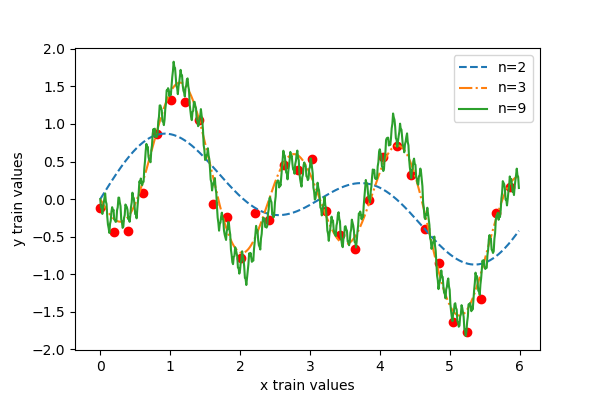
\includegraphics[width=0.7\textwidth]{img/3c.png} 
	\end{center}
	
	\pythonexternal{src/a13c.py}
	\end{answer}
		
	\end{question}
	
	
	%----------------------------------------------
	
	\begin{question}{Training a Model}{2}
		The root mean square error (RMSE) is defined as $\text{RMSE} = \sqrt{\frac{1}{N}\sum_{i=1}^{N}(y^{\text{true}}_i-y^{\text{predicted}}_i)^{2}}$, where $N$ is the number of data points. 
		Using the LLS algorithm implemented in the previous exercise, train a different model for each of the number of features between 1 and 9, i.e.,  [1,2,3...,9].
		For each of these models compute the corresponding RMSE for the training set. 
		Attach a plot where the x-axis represents the number of features and the y-axis represents the RMSE.
		
\begin{answer}
	\begin{center}
		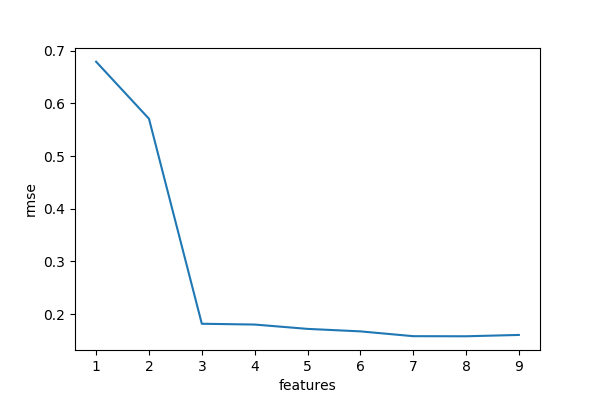
\includegraphics[width=0.5\textwidth]{img/3d.png} 
	\end{center}
	
		\pythonexternal{src/a13d.py}	
\end{answer}
		
	\end{question}
	
	
	%----------------------------------------------
	
	\begin{question}{Model Selection}{4}
		Using the models trained in the previous exercise, compute the RMSE of each of these models for the validation set.\\
		Compare in one plot the RMSE on the training set and on the validation set. 
		How do they differ? 
		Can you explain what is the reason for these differences? (Hint: remember the plot from Exercise~c)~) 
		What is the number of features that you should use to achieve a proper modeling?
		
	\begin{answer}
	Note: Use the parameters $a_i$ from c) on the validation dataset!
\begin{figure}[H]
	\centering
	\begin{minipage}{.5\textwidth}
		\centering
		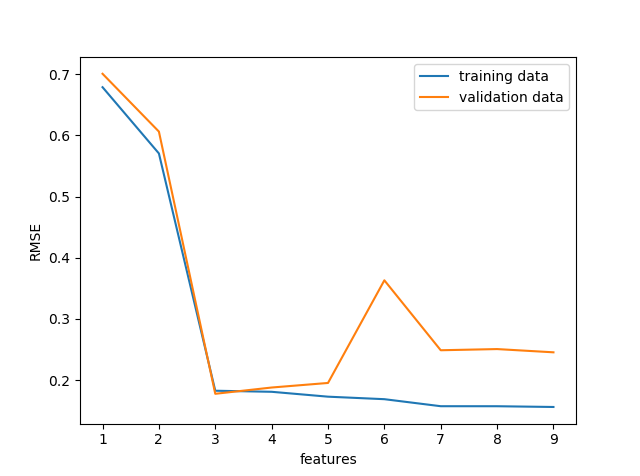
\includegraphics[width=1\textwidth]{img/3e.png} 
		\captionof{figure}{Comparing RMSE }
		\label{fig:test1}
	\end{minipage}%
	\begin{minipage}{.5\textwidth}
		\centering
		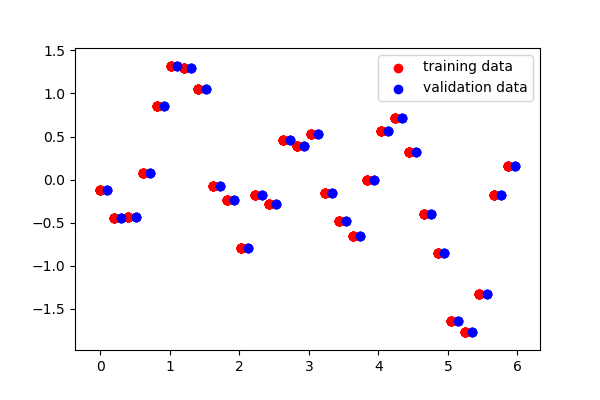
\includegraphics[width=1\textwidth]{img/data.png} 
		\captionof{figure}{Data sets}
		\label{fig:test2}
	\end{minipage}
\end{figure}

	
	How do they differ:\\
	Using 3 features the training set and the validation set have have the same rmse. Afterwards the rmse of the training set is marginally decreasing and the rmse of the validation set is increasing. 
	
	What is the reason for these differences:\\
	Using three features the model is sufficiently described (see e.g c). If you use more features the model is overfitted. Thus the rmse is increasing
	
	
	What is the number of features that you should use to achieve a proper modeling:\\
	As you can see in figure 29 the smallest rmse is reached for 3 features. For this reason 3 features should be used.

	\pythonexternal{src/a13e.py}
	\end{answer}
	\end{question}
	
	%----------------------------------------------
	
	\begin{question}{Cross Validation}{8}
		$K$-fold cross validation is a common approach to estimate the test error when the dataset is small.
		The idea is to randomly divide the training set into $K$ different datasets.
		Each of these datasets is then used as validation set for the model trained from the remaining $K-1$ datasets.
		The resulting vector of errors $\vec E = [ e_1... e_K ]$ can now be used to compute a distribution (typically by fitting a Gaussian distribution).
		When $K$ is equal to the number of data points, $K$-fold cross validation takes the name of leave-one-out cross validation (LOO).
		
		Apply LOO using only the training set and compute the mean/variance of the RMSE for the learned models. 
		Repeat for the models with the number of features between 1 and 9, i.e.,  [1,2,3...,9]
		
		Attach a plot showing the mean/variance (as a distribution) of the RMSE computed using LOO and having on the x-axis the number of features and on the y-axis the RMSE.
		Which is the optimal number of features now? 
		Discuss the results obtained and compare against model selection using train/validation set.
		
\begin{answer}
	\begin{center}
		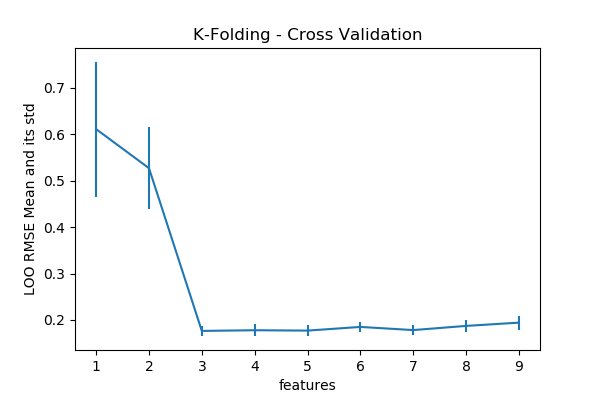
\includegraphics[width=0.7\textwidth]{img/3f.png} 
	\end{center}
	
	\pythonexternal{src/a13f.py}

	
	\end{answer}
	\end{question}
	
	
	
	%----------------------------------------------
	
	
	\begin{question}{Kernel Functions}{2}
		A kernel function $k(\vec{\mbox{x}}_{i},\vec{\mbox{x}}_{j})$ is given by the inner product of two feature vectors. Write out the kernel function for the previous set of features where $n=3$.
		
	\begin{answer}
	
		$k(x_i,x_j)_{n=3}=\begin{bmatrix}
		sin(x_i)&sin(2x_i)&sin(4x_i)
		\end{bmatrix}
		\begin{bmatrix}
			sin(x_j)\\sin(2x_j)\\sin(4x_j)
		\end{bmatrix}=sin(x_i)sin(x_j)+sin(2x_i)sin(2x_j)+sin(4x_i)sin(4x_j)$

	References:\\
	\hyperlink{https://de.wikipedia.org/wiki/Kernel\_(Maschinelles\_Lernen)}{https://de.wikipedia.org/wiki/Kernel\_(Maschinelles\_Lernen)}
	
	\hyperlink{https://en.wikipedia.org/wiki/Kernel\_(statistics)}{		https://en.wikipedia.org/wiki/Kernel\_(statistics)}
	

	\end{answer}
	\end{question}
	
	
	%----------------------------------------------
	
	\begin{question}{Kernel Regression}{6}
		
		The kernel function in the previous question required explicit definition of the type and number of features, which is often difficult in practice. Instead, we can use a kernel that defines an inner product in a (possibly infinite dimensional) feature space. \\
		Using the training set and an exponential squared kernel 		$k( \vec{x}_{i} , \vec{x}_{j} )= \exp ( -\frac{1}{\sigma^{2}} \Vert \vec{x}_{i}-\vec{x}_{j}\Vert ^{2} )$ with $\sigma=0.15$, predict output values $y$ for input values $x\in\{0,0.01,\ldots,6\}$. Attach a plot of your results.
		\\
		(Hint: use standard kernel regression: $f(\mbox{\ensuremath{\vec{x}}})=\vec{k}\T\vec{K}^{-1}\vec{y}$ with $\vec{K}_{ij}=k(\vec{x}_{i},\vec{x}_{j})$ and $\vec{k}_{i}=k(\vec{x},\vec{x}_{i})$).
		
		Compute the RMSE on the validation set for the kernel regression model. Compare it with the RMSE of the best LLS model you found.
		
\begin{answer}
	Some Theory:
	\begin{itemize}
		\item squared Euclidean distance: $|| a - b||^2 = \sqrt{ (a_1-b_1)^2+...+(a_n-b_n)^2}^2 =  (a_1-b_1)^2+...+(a_n-b_n)^2$
		\item Kernel function: $k(x_1,x_2)=\phi(x_1)^T \phi(x_2), \quad (\text{inner product})$
		\item Kernel regression: $y_{pred} = f(x_{\text{pred}})=k^T_{\text{pred, dataset}} K^{-1}_{\text{dataset}} y_{\text{dataset}}$
		\item $k_i=k(x,x_i)=[e^{- \frac{||x_{pred}- x_{0,dataset} ||^2}{\sigma^2}}, ... ,e^{- \frac{||x_{pred}- x_{n,dataset} ||^2}{\sigma^2}}], \quad \text{Gaussian Radial Basis kernel function} $
		\item $K_{ij}=k(x_i,x_j)=\begin{bmatrix}
		e^{- \frac{||x_{0,dataset}- x_{0,dataset} ||^2}{\sigma^2}}&...&e^{- \frac{||x_{n,dataset}- x_{0,dataset} ||^2}{\sigma^2}}\\...&...&...\\e^{- \frac{||x_{0,dataset}- x_{n,dataset} ||^2}{\sigma^2}}&...&e^{- \frac{||x_{n,dataset}- x_{n,dataset} ||^2}{\sigma^2}}
		\end{bmatrix}$
	\end{itemize}
	\begin{figure}[H]
		\centering
		\begin{minipage}{.5\textwidth}
			\centering
				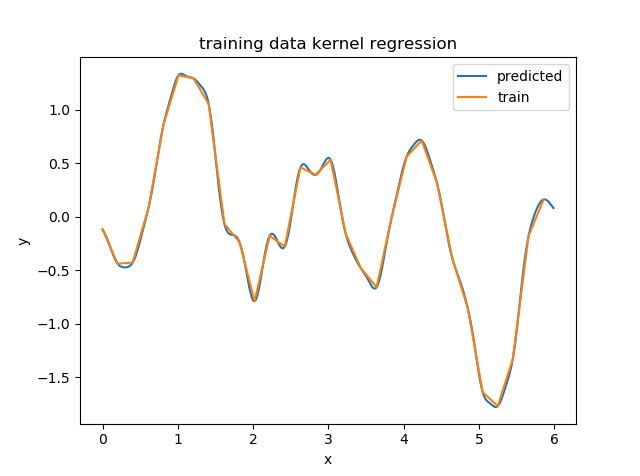
\includegraphics[width=1\textwidth]{img/3g.png} 
		\end{minipage}%
		\begin{minipage}{.5\textwidth}
			\centering
			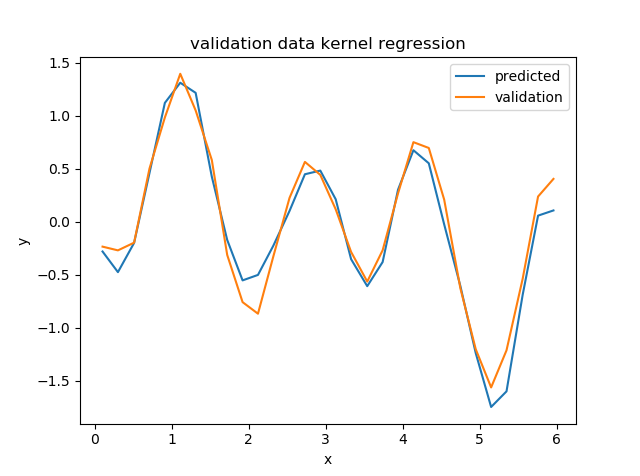
\includegraphics[width=1\textwidth]{img/3g2.png} 
		\end{minipage}
	\end{figure}
	
	
		The prediction for the training data is nearly perfect. You can see no difference between the prediction and the rail data. But th prediction for the validation data is not so well, you can see big differences for $x=2$. The calculated RMSE is 0.2422. So it is slightly bigger compared to the Linear Regression model with three features.
		
		\pythonexternal{src/a13g.py}
	
	Refererences:\\
	\url {https://en.wikipedia.org/wiki/Radial_basis_function_kernel}
	
	\end{answer}
	\end{question}
	
	
	%----------------------------------------------
	
	\begin{question}[bonus]{Derivation}{5}
		Explain the concept of ridge regression and why/when it is used.
		Derive its final equations presented during the lecture.\\
		(Hint: remind that for normal linear regression the cost function is $J = \frac{1}{2}\sum_{i=1}^N ( f(\vec x_i) - y_i ) ^2 \,$ )\\
		(Hint 2: use matrix notation)
		
\begin{answer}
		
		Ordinary Linear Squares (OLS):
		\begin{itemize}
			\item Parameters $\Theta$ are Best linear unbiased estimators (BLUE).
			\item The Parameters have the smallest variance out of all other unbiased estimators.
			\item If 2 or more parameters are highly correlated the variance is quite high and quite different solution's occur for different data sets. In such a case Ridge Regression should be used! 
			\item $f_{\Theta}=\phi^T(x_i) \Theta$
			\item $J=\frac{1}{2} \sum_{i=1}^{N} (y_i - f_{\Theta}(x_i))^2, \quad J=\frac{1}{2}(Y-\Phi \Theta)^T (Y-\Phi \Theta)$
			\item $\Theta = (\Phi^T \Phi)^{-1} \Phi^T Y$
		\end{itemize}
		\bigskip
		Ridge ("Kamm") Regression:
		\begin{itemize}
			\item Estimators are biased and can therefore have an even lower variance compared to OLS.
			\item Especially if the parameters are highly correlated ridge regression is a powerful method to restrict the correlation of the parameters using a 
			lagrangian multiplier $\lambda$.
			\item $min_\Theta ||y-\Phi \Theta||^2_2+\lambda ||\Theta||^2_2 $
			\item $J=\frac{1}{2} [ \sum_i^N (y_i \phi(x_i) \Theta)^2+\lambda \Theta^T \Theta], \quad J=\frac{1}{2}[(Y-\Phi \Theta)^T (Y-\Phi \Theta)+\lambda \Theta^T \Theta],\quad \frac{\partial J}{\partial \Theta}=0$
			\item $J=\frac{1}{2}[Y^T Y-Y^T \Phi \Theta - \Phi^T \Theta^T Y + \Phi^T \Theta^T \Phi \Theta+\lambda \Theta^T \Theta] = \frac{1}{2}[Y^T Y-2Y^T \Phi \Theta+ \Phi^T \Theta^T \Phi \Theta+\lambda \Theta^T \Theta]$
			\item $\frac{\partial J}{\partial \Theta}=Y^T \Phi - \Phi^T \Phi \Theta +\lambda \Theta = 0, \quad \Phi^T Y = (\Phi^T \Phi + \lambda I) \Theta$
			\item $\Theta = (\Phi^T \Phi+\lambda I)^{-1} \Phi^T Y$
		\end{itemize}
		
				\begin{center}
					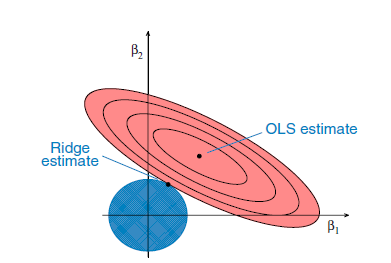
\includegraphics[width=0.7\textwidth]{img/ridge.png} 
				\end{center}

		
		\url{https://www.youtube.com/watch?v=5asL5Eq2x0A}\\
		\url{https://onlinecourses.science.psu.edu/stat857/node/155}
	\end{answer}
	
	
	\end{question}	
	
\end{questions}

